\documentclass[aspectratio=149, dvipsnames]{beamer}
% \documentclass[aspectratio=149, dvipsnames, handout]{beamer}
\usetheme{Inf}
\usepackage{xcolor}
\usepackage[T1]{fontenc}
\usepackage[utf8]{inputenc}

\usepackage{pifont}
\usepackage{venturis}

\setlength{\parskip}{.3em}
\usepackage{indentfirst}

\usepackage{amssymb}
\usepackage{amsmath}
\usepackage{mathtools}
\usepackage{booktabs}
\usepackage{graphicx}
\usepackage{xparse}
\usepackage{multirow}
\usepackage{tabularx}

\usepackage{tikz}
\usetikzlibrary{positioning, arrows.meta, fit, shapes.misc, calc}
% Estilo neutro (caso seja útil em outro lugar)
\tikzstyle{pipebox}=[draw, very thick, rounded corners, minimum height=10mm, minimum width=20mm, align=center, font=\small]
% Estilos coloridos por estágio (usados no roadmap)
\tikzstyle{databox}=[draw, very thick, rounded corners, minimum height=12mm, minimum width=22mm, align=center, font=\small, fill=blue!10, draw=blue!50!black]
\tikzstyle{modelbox}=[draw, very thick, rounded corners, minimum height=12mm, minimum width=22mm, align=center, font=\small, fill=green!12, draw=green!50!black]
\tikzstyle{evalbox}=[draw, very thick, rounded corners, minimum height=12mm, minimum width=22mm, align=center, font=\small, fill=orange!15, draw=orange!60!black]
\tikzstyle{pipearrow}=[-{Stealth[length=2.5mm]}, very thick]

% Permite "visible on=<n->" em nós e setas TikZ (compatível com overlays do Beamer).
\tikzset{
  invisible/.style={opacity=0},
  visible on/.style={alt={#1{}{invisible}}},
  alt/.code args={<#1>#2#3}{%
    \alt<#1>{\pgfkeysalso{#2}}{\pgfkeysalso{#3}}%
  },
}

\usepackage{macros}

% ============================================================
% Tamanho dos logos do slide "Two readings of power" (Archidekt / calculadora).
% ============================================================
\newcommand{\readlogoheight}{1.1cm}

% Tamanho dos mini-logos (Archidekt / EDHPowerLevel) no slide "Data collection".
\newcommand{\sourcelogoheight}{0.75cm}

% ============================================================
% Title page
% ============================================================
\title
[
    \textbf{Commander bracket divergence}
]
{
    Modeling Divergence Between Community-Perceived\\
    and Automatically Calculated MTG Commander Brackets
}

\author
[
    Massuquetti \& Chitolina
]
{
    \centering \footnotesize\textcolor{darkgray}{} \\[-7pt]
}

\institute
{
    \small \textcolor{black}{Henrique Bidarte Massuquetti} \\[-2pt]
    \small \textcolor{black}{Marco Antônio Chitolina da Silva} \\[-8pt]
}

\date
{
    \textcolor{black}{CMP263 -- Machine Learning} \\[-2pt]
    \textcolor{black}{Prof.~Mariana Recamonde Mendoza} \\[-2pt]
    Federal University of Rio Grande do Sul
}

\AtBeginSection
{
    \setbeamercolor{footline}{fg=InfWhite}
    \begin{frame}[noframenumbering]
        \begin{huge}
            \begin{center}
                \insertsection
            \end{center}
        \end{huge}
    \end{frame}
    \setbeamercolor{footline}{fg=InfBlack}
}

\begin{document}

% ============================================================
% Cover
% ============================================================
\InfTitlePage
\setbeamercolor{footline}{fg=InfBlack}


\section{Introduction.}

% ============================================================
% SLIDE 1 -- MTG and Commander (imagem aparece ANTES dos bullets)
% NOTA: ~50s.
% Sequência de cliques: (1) imagem do logo do Magic/Commander, (2-5) bullets.
% O QUE FALAR: MTG (1993): card game; player monta um deck e gasta mana;
% formato Commander: multiplayer, 100 cartas, comandante lendária; sem
% matchmaking, equilíbrio vem da conversa pré-jogo.
% ============================================================
\begin{frame}{Magic: The Gathering and Commander.}
    \begin{columns}
        \begin{column}{.58\textwidth}
            \begin{itemize}
                \item<3-> \textbf{MTG} (1993): collectible card game. Each player builds a \textit{deck} and casts cards by paying \textit{mana} to defeat opponents.
                \item<4-> The game has many \textbf{formats} (rule sets). We study \textbf{Commander}.
                \item<5-> \textbf{Commander}: \textit{multiplayer} (4 players), 100-card deck (one copy of each), led by a legendary \textbf{commander}.
                \item<6-> \textbf{No matchmaking}: balance comes from a \textit{pre-game} conversation.
            \end{itemize}
        \end{column}%
        \hfill%
        \begin{column}{.38\textwidth}
            \visible<2->{\begin{center}
                
\includegraphics[width=\textwidth]{figures/mtg-commander-logo.jpg}
            \end{center}}
        \end{column}
    \end{columns}
\end{frame}


% ============================================================
% SLIDE 2 -- Commander Brackets (oficial infographic)
% NOTA: ~45s. Texto introdutório -> imagem -> texto final.
% ============================================================
\begin{frame}{Commander Brackets.}
    \visible<2->{{\small \textbf{Brackets} (scale 1--5): the official vocabulary for that conversation. When publishing a deck, the author picks the bracket that best describes its power level.}}
    \visible<3->{\begin{center}
        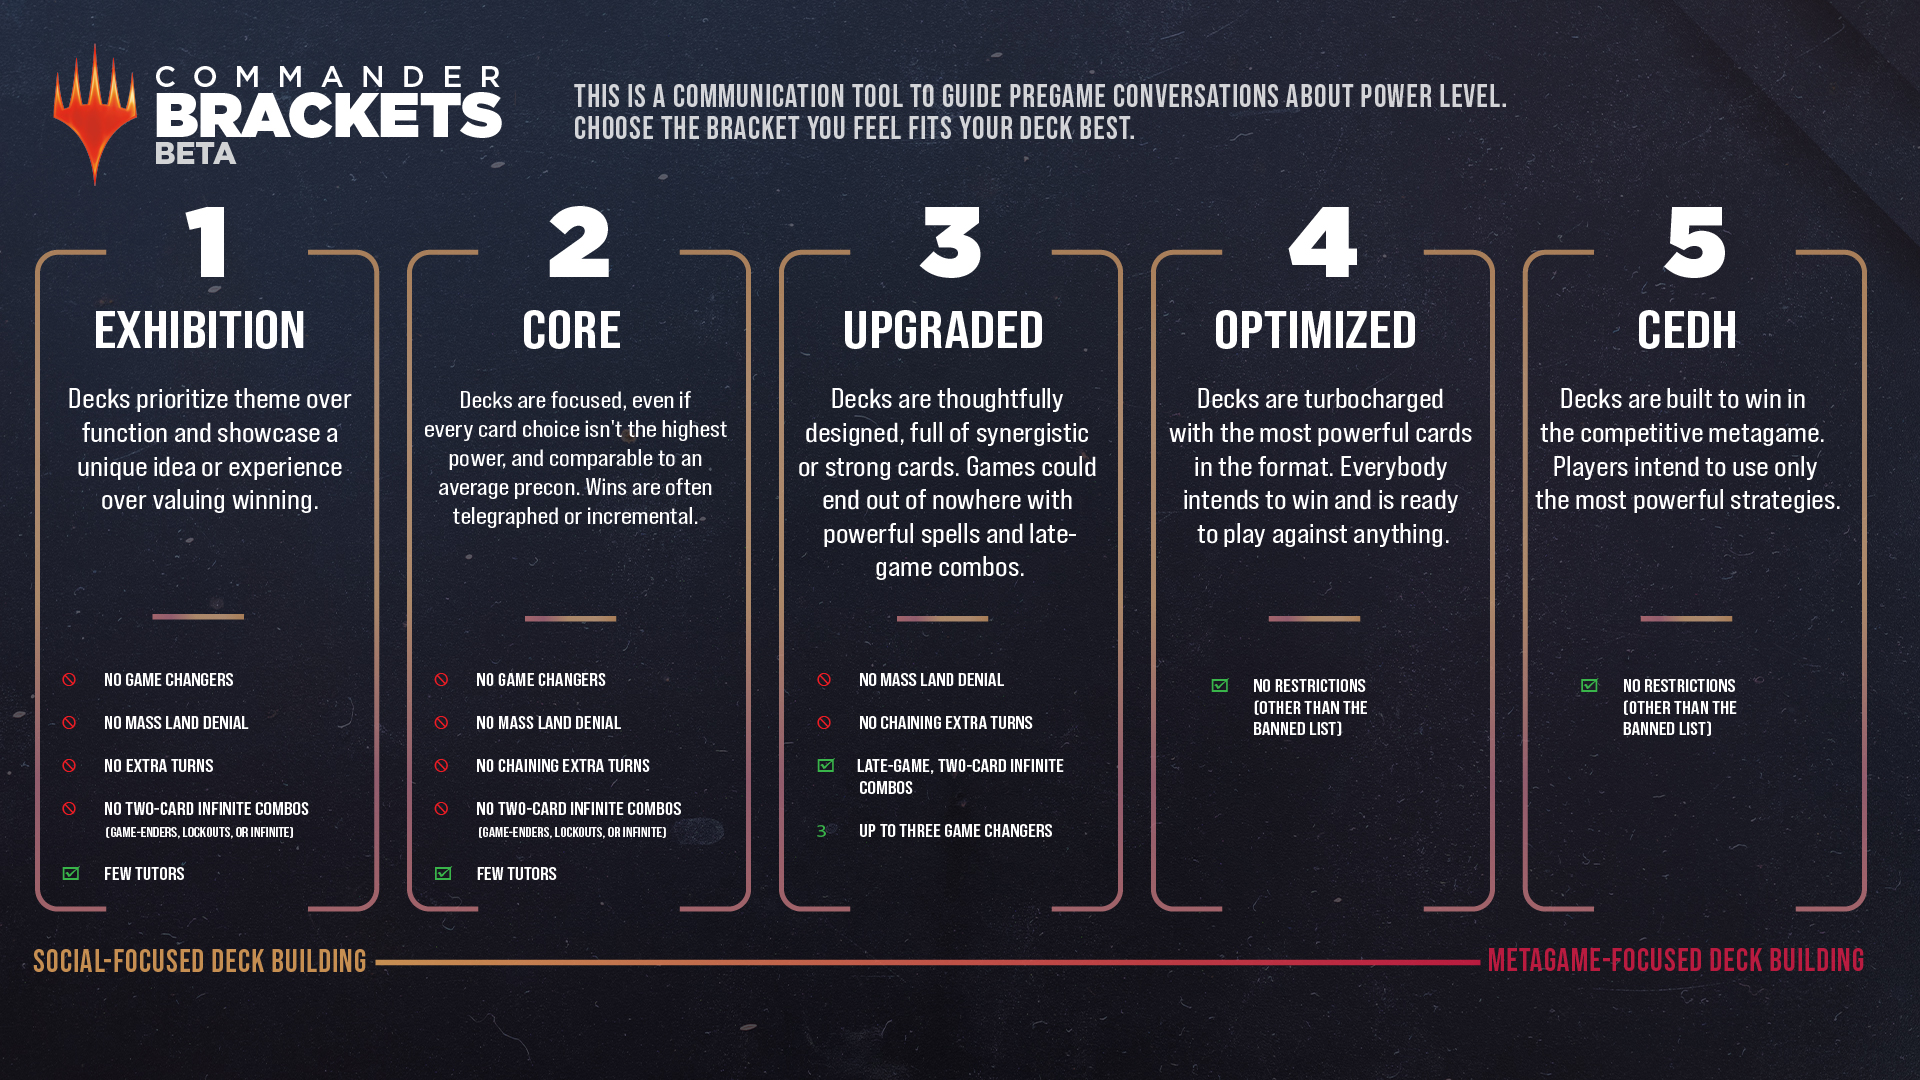
\includegraphics[width=0.62\textwidth]{figures/commander-brackets.jpg}
    \end{center}}
    \visible<4->{{\small We focus on the middle --- \textbf{brackets 2--4} --- where almost all the public data lives and where the actual negotiation happens (1 and 5 are the extremes: thematic and cEDH).}}
\end{frame}


% ============================================================
% SLIDE 3 -- Two readings of power
% NOTA: ~40s. Coluna esquerda (Comunidade): título -> bullet 1 -> bullet 2
% -> logo Archidekt. Coluna direita (Calculadora): mesmo padrão. Frase final.
% ============================================================
\begin{frame}{Two readings of power.}
    \begin{columns}[t]
        \begin{column}{.45\textwidth}
            \visible<2->{\textbf{Community ($y_{\text{arch}}$).}}
            \begin{itemize}
                \item<3-> Bracket the author picks when publishing the deck on Archidekt.
                \item<4-> \textit{Subjective}: varies between players.
            \end{itemize}
        \end{column}%
        \hfill%
        \begin{column}{.45\textwidth}
            \visible<6->{\textbf{Calculator ($y_{\text{calc}}$).}}
            \begin{itemize}
                \item<7-> Bracket EDHPowerLevel returns for the same decklist.
                \item<8-> \textit{Deterministic}: same input $\Rightarrow$ same output.
            \end{itemize}
        \end{column}
    \end{columns}
    \vspace{0.5cm}
    % Cada logo no seu próprio clique, depois dos bullets de cada lado.
    \begin{columns}
        \begin{column}{.45\textwidth}
            \centering
            \visible<5->{
\includegraphics[height=\readlogoheight]{figures/archidekt-logo.png}}
        \end{column}%
        \hfill%
        \begin{column}{.45\textwidth}
            \centering
            \visible<9->{
\includegraphics[height=\readlogoheight]{figures/calculator-logo.png}}
        \end{column}
    \end{columns}
    \vfill
    \visible<10->{\begin{center}\Large \textbf{They frequently disagree.}\end{center}}
\end{frame}


% ============================================================
% SLIDE 4 -- Research question
% NOTA: ~45s.
% ============================================================
\begin{frame}{Our research question.}
    \visible<2->{%
    \begin{quote}
        \large\textit{``To what extent do Archidekt-assigned Commander brackets diverge from automatically calculated bracket estimates, and which deck characteristics explain that disagreement?''}
    \end{quote}}
    \bigskip
    \visible<3->{\textbf{We don't want to arbitrate.} We want to \textit{describe} where the misalignment lies.}
    \bigskip

    \visible<4->{\textbf{Why it matters:}}
    \begin{itemize}
        \item<5-> Real problem for the Commander community.
        \item<6-> Case study of divergence between a human label and a heuristic label.
    \end{itemize}
\end{frame}


\section{Methodology.}


% ============================================================
% SLIDE 5 -- Roadmap (cores por estágio, sem a frase "Pipeline em ordem")
% NOTA: ~60s. Cada caixa em um clique (8 caixas).
% Cores: Data (azul), Modeling (verde), Evaluation (laranja).
% ============================================================
\begin{frame}{Roadmap.}
    \vfill
    \begin{center}
        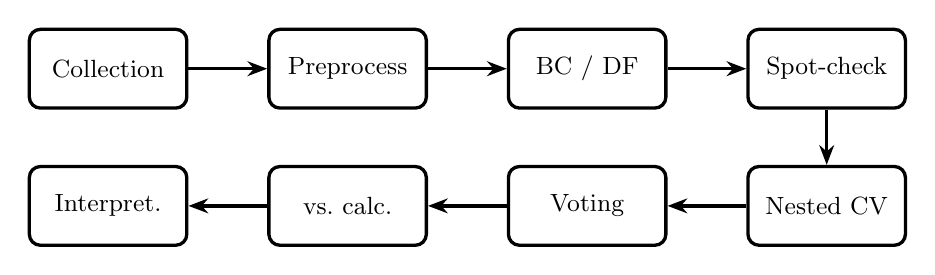
\begin{tikzpicture}[node distance=7mm and 10mm]
            % Linha 1: esquerda -> direita
            \node[pipebox, visible on=<2->] (col)  {Collection};
            \node[pipebox, right=of col,  visible on=<3->] (prep) {Preprocess};
            \node[pipebox, right=of prep, visible on=<4->] (rep)  {BC / DF};
            \node[pipebox, right=of rep,  visible on=<5->] (spot) {Spot-check};
            % Linha 2: direita -> esquerda
            \node[pipebox, below=of spot, visible on=<6->] (cv)  {Nested CV};
            \node[pipebox, left=of cv,    visible on=<7->] (vot) {Voting};
            \node[pipebox, left=of vot,   visible on=<8->] (cmp) {vs.\ calc.};
            \node[pipebox, left=of cmp,   visible on=<9->] (int) {Interpret.};

            \draw[pipearrow, visible on=<3->] (col)  -- (prep);
            \draw[pipearrow, visible on=<4->] (prep) -- (rep);
            \draw[pipearrow, visible on=<5->] (rep)  -- (spot);
            \draw[pipearrow, visible on=<6->] (spot) -- (cv);
            \draw[pipearrow, visible on=<7->] (cv)   -- (vot);
            \draw[pipearrow, visible on=<8->] (vot)  -- (cmp);
            \draw[pipearrow, visible on=<9->] (cmp)  -- (int);
        \end{tikzpicture}
    \end{center}
    \vfill
\end{frame}


\section{Data.}

% ============================================================
% SLIDE 6 -- Data collection (filtros como sub-bullets)
% NOTA: ~45s.
% Sequência: logo Archidekt -> "Public REST API" -> "Filters:" -> 4 sub-bullets
% -> logo Calc -> "No public API" -> "Playwright + Chromium..." -> tabela funil.
% ============================================================
\begin{frame}{Data collection.}
    \begin{columns}
        \begin{column}{.55\textwidth}
            \visible<2->{
\includegraphics[height=\sourcelogoheight]{figures/archidekt-logo.png}}
            \begin{itemize}
                \item<3-> Public paginated REST API.
                \item<4-> Filters:
                \begin{itemize}\footnotesize
                    \item<5-> Commander format
                    \item<6-> $\geq$ 1{,}000 views
                    \item<7-> brackets $\in \{2,3,4\}$
                    \item<8-> 100-card mainboard
                \end{itemize}
            \end{itemize}
            \medskip
            \visible<9->{
\includegraphics[height=\sourcelogoheight]{figures/calculator-logo.png}}
            \begin{itemize}
                \item<10-> No public API.
                \item<11-> Playwright + headless Chromium: paste decklist, read bracket from DOM.
            \end{itemize}
        \end{column}%
        \hspace{0.3cm}%
        \begin{column}{.32\textwidth}
            \visible<12->{\begin{center}\footnotesize
                \setlength{\tabcolsep}{4pt}
                \begin{tabular}{rl}
                \toprule
                14{,}421 & decks collected \\
                $-$1{,}471 & duplicates \\
                $-$815 & $y_{\text{calc}} \in \{1,5\}$ \\
                \midrule
                \textbf{12{,}135} & \textbf{modeling set} \\
                \bottomrule
                \end{tabular}
            \end{center}}
        \end{column}
    \end{columns}
\end{frame}


% ============================================================
% SLIDE 7 -- How large is the divergence?
% NOTA: ~50s. Figura da matriz de concordância -> 3 headlines.
% ============================================================
\begin{frame}{How large is the divergence?}
    \begin{columns}[c]
        \begin{column}{.52\textwidth}
            \visible<2->{\begin{center}
                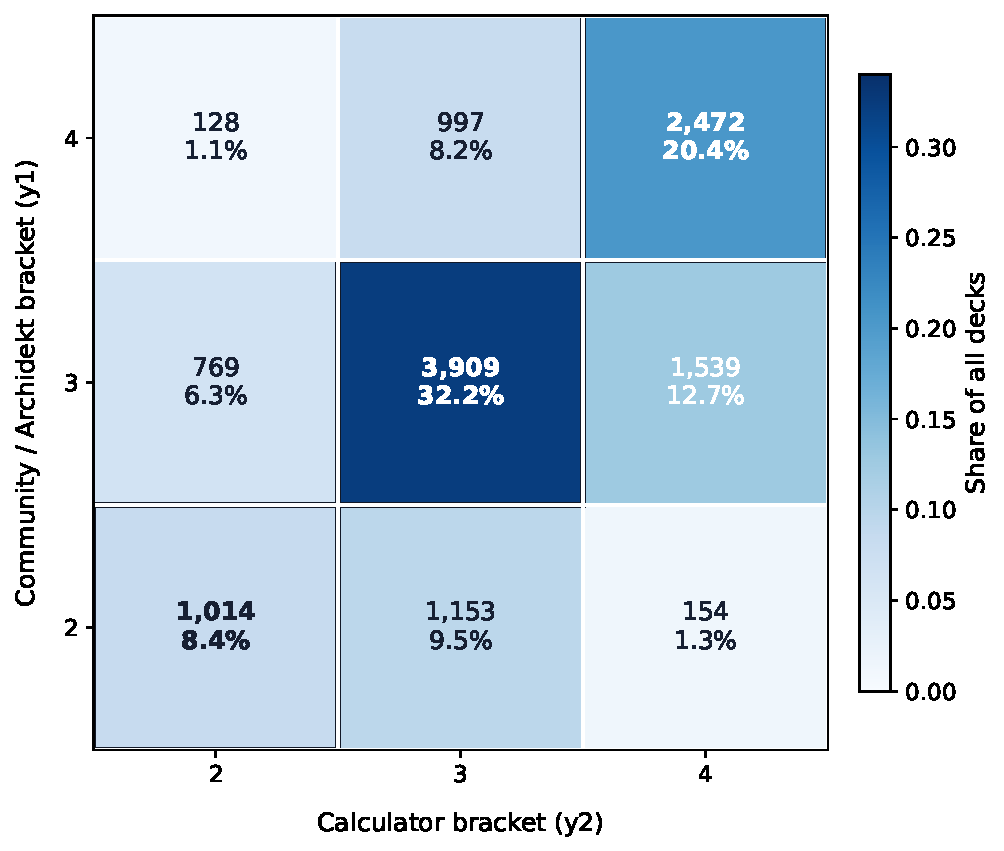
\includegraphics[width=\textwidth]{figures/agreement_matrix_y1_y2.pdf}
            \end{center}}
        \end{column}%
        \hspace{0.2cm}%
        \begin{column}{.42\textwidth}
            \small
            \begin{itemize}
                \item<3-> \textbf{60.9\%} exact agreement.
                \item<4-> \textbf{97.7\%} within $\pm 1$ bracket.
                \item<5-> When they disagree, the calculator rates:
                \begin{itemize}\footnotesize
                    \item<6-> \textbf{higher} in 23.5\%
                    \item<7-> \textbf{lower} in 15.6\%
                \end{itemize}
            \end{itemize}
        \end{column}
    \end{columns}
\end{frame}


% ============================================================
% SLIDE 8 -- Two representations (imagens alinhadas com seus blocos)
% NOTA: ~50s. Imagem BC fica no quadrante superior direito (com bullets BC).
% Imagem DF fica no quadrante inferior direito (com bullets DF). Para isso,
% adicionamos vspace entre as imagens.
% ============================================================
\begin{frame}{Two representations of the same deck.}
    \begin{columns}[t]
        \begin{column}{.5\textwidth}
            \begin{itemize}
                \item<2-> \textbf{Bag of Cards (BC).}
                \begin{itemize}
                    \item<3-> Sparse vector indexed by card ($\approx$ 11k dim).
                    \item<4-> Hypothesis: community reacts to \textit{specific cards}.
                \end{itemize}
                \medskip
                \item<6-> \textbf{Deck Features (DF).}
                \begin{itemize}
                    \item<7-> Dense vector of 102 structural attributes.
                    \item<8-> Mana curve, Game Changers, tutors, combos, price, etc.
                    \item<9-> Hypothesis: community reacts to \textit{aggregate structure}.
                \end{itemize}
            \end{itemize}
        \end{column}%
        \hfill%
        \begin{column}{.45\textwidth}
            \visible<5->{\begin{center}
                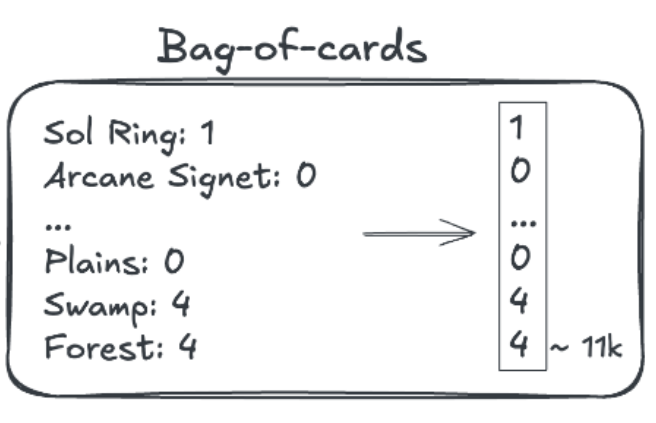
\includegraphics[width=0.85\linewidth]{figures/mtg-bag-of-cards.png}
            \end{center}}
            \visible<10->{\begin{center}
                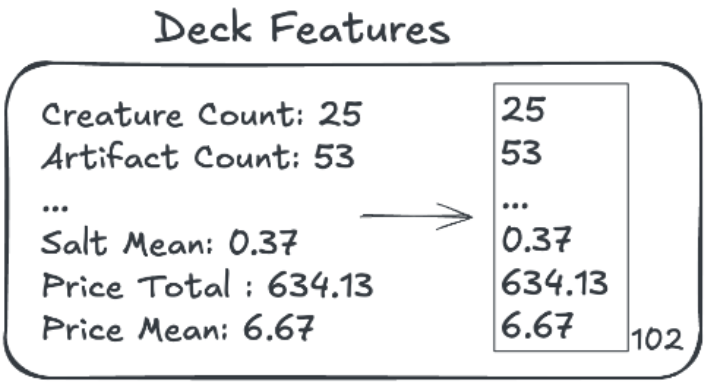
\includegraphics[width=0.85\linewidth]{figures/mtg-deck-features.png}
            \end{center}}
        \end{column}
    \end{columns}
\end{frame}


\section{Results.}

% ============================================================
% SLIDE 9 -- Spot-checking (disposição melhorada)
% NOTA: ~50s. Tabela primeiro, depois uma única frase de fechamento.
% ============================================================
\begin{frame}{Spot-checking.}
    \vfill
    \visible<2->{\begin{center}\scriptsize
        \begin{tabular}{lrcrcc}
            \toprule
            Algorithm & DF & rank & BC & rank & in $A_{\text{union}}$ \\
            \midrule
            Gradient Boosting   & 0.6850 & 1 & 0.6342 & 1 & \checkmark \\
            Random Forest       & 0.6686 & 2 & 0.5243 & 6 & \checkmark \\
            Logistic Regression & 0.6672 & 3 & 0.5927 & 2 & \checkmark \\
            Linear SVC          & 0.6225 & 4 & 0.5459 & 4 & \checkmark \\
            Decision Tree       & 0.6042 & 5 & 0.5445 & 5 & \checkmark \\
            Naive Bayes         & 0.5792 & 6 & 0.5570 & 3 & \checkmark \\
            KNN                 & 0.5241 & 7 & 0.4541 & 7 & --- \\
            \bottomrule
        \end{tabular}
    \end{center}}
    \vfill
    \visible<3->{\begin{center}\textbf{KNN drops.}\end{center}}
    \visible<4->{\begin{center}The 6 remaining algorithms $\times$ 2 representations $=$ \textbf{12 models} for nested CV.\end{center}}
    \vfill
\end{frame}


% ============================================================
% SLIDE 10 -- Nested CV (texto reduzido)
% NOTA: ~75s. Tabela + 1 headline. Tirei o cabeçalho metodológico e a linha de
% sanidade extra para o slide ficar mais leve.
% ============================================================
\begin{frame}{Nested CV: DF beats BC for every algorithm.}
    \vfill
    \visible<2->{\scriptsize
    \setlength{\tabcolsep}{4pt}
    \begin{center}
        \begin{tabular}{l|rrc|rrc}
            \toprule
            & \multicolumn{3}{c|}{DF} & \multicolumn{3}{c}{BC} \\
            Algorithm & Macro-F1 & Acc. & rank & Macro-F1 & Acc. & rank \\
            \midrule
            Gradient Boosting   & $0.6908 \pm 0.009$ & 0.698 & 1 & $0.6433 \pm 0.012$ & 0.644 & 1 \\
            Random Forest       & $0.6733 \pm 0.008$ & 0.703 & 2 & $0.6326 \pm 0.012$ & 0.653 & 2 \\
            Decision Tree       & $0.6727 \pm 0.010$ & 0.688 & 3 & $0.5475 \pm 0.012$ & 0.554 & 6 \\
            Logistic Regression & $0.6707 \pm 0.011$ & 0.694 & 4 & $0.6236 \pm 0.010$ & 0.621 & 3 \\
            Linear SVC          & $0.6557 \pm 0.009$ & 0.658 & 5 & $0.6147 \pm 0.012$ & 0.628 & 4 \\
            Naive Bayes         & $0.5905 \pm 0.009$ & 0.587 & 6 & $0.5535 \pm 0.009$ & 0.564 & 5 \\
            \bottomrule
        \end{tabular}
    \end{center}
    \normalsize}
    \vfill
    \visible<3->{\begin{center}\textbf{DF $>$ BC} in every algorithm.\end{center}}
    \visible<4->{\begin{center}Best: \textbf{DF Gradient Boosting, F1 $=$ 0.6908}.\end{center}}
    \vfill
\end{frame}


% ============================================================
% SLIDE 11 -- Comparison with the calculator
% NOTA: ~75s. Tabela, depois explicações progressivas das colunas.
% ============================================================
\begin{frame}{Comparison with the calculator.}
    \visible<2->{\scriptsize
    \setlength{\tabcolsep}{3pt}
    \begin{center}
        \begin{tabular}{@{}llrrrr@{}}
            \toprule
            Case & Source & Exact & $\pm 1$ & F1 calc & F1 arch \\
            \midrule
            Raw labels & $y_{\text{arch}}$ & 60.9\% & 97.7\% & 0.5843 & --- \\
            Max agreement & DF RF & 69.3\% & 99.5\% & 0.6674 & 0.6733 \\
            Min agreement & BC DT & 54.2\% & 96.6\% & 0.5328 & 0.5475 \\
            Best individual & DF GB & 64.0\% & 98.1\% & 0.6323 & 0.6908 \\
            Best BC & BC GB & 60.3\% & 97.3\% & 0.5984 & 0.6433 \\
            Best ensemble & Top-3 vote & 66.7\% & 98.7\% & 0.6499 & 0.6941 \\
            \bottomrule
        \end{tabular}
    \end{center}
    \normalsize}
    \medskip

    \visible<3->{{\footnotesize $y_{\text{calc}}$ was \textbf{never used in training} --- this is a purely descriptive comparison.}}
    \vfill
\end{frame}


% ============================================================
% SLIDE 11b -- Agreement matrices
% NOTA: ~40s na figura.
% ============================================================
\begin{frame}{Where does the disagreement go?}
    \visible<2->{\begin{center}
        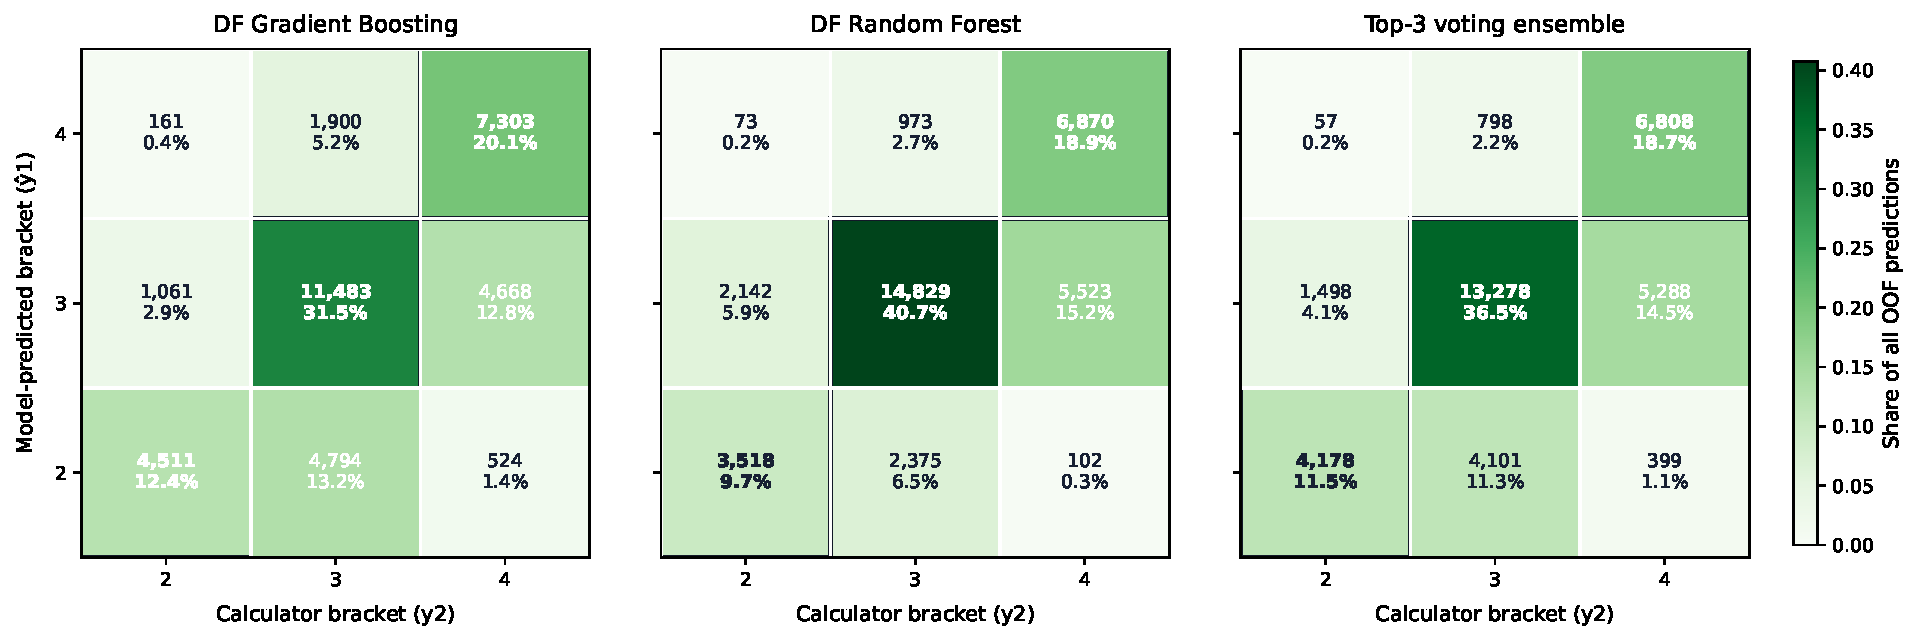
\includegraphics[width=\textwidth]{figures/agreement_matrix_df_models_pred_y2.pdf}
    \end{center}}
    \visible<3->{{\footnotesize All three predictors sit \textbf{below} the calculator more often than above it --- the same asymmetry seen in the raw community labels.}}
\end{frame}


% ============================================================
% SLIDE 12 -- Interpretability
% NOTA: ~60s. Cada coluna em um clique; tabelas em outro clique; frase final.
% ============================================================
\begin{frame}{Interpretability.}
    \begin{columns}
        \begin{column}{.44\textwidth}
            \visible<2->{\textbf{DF Gradient Boosting} \\ {\footnotesize\textit{permutation importance}}}
            \visible<3->{\begin{center}
                \footnotesize
                \begin{tabular}{lr}
                    \toprule
                    Feature & PI \\
                    \midrule
                    \texttt{game\_changer\_count} & \textbf{0.228} \\
                    \texttt{mass\_land\_denial\_count} & 0.029 \\
                    \texttt{unique\_atomic\_combo\_refs} & 0.014 \\
                    \texttt{tutor\_count} & 0.010 \\
                    \texttt{cmc\_1\_count} & 0.006 \\
                    \bottomrule
                \end{tabular}
            \end{center}}
        \end{column}%
        \hfill%
        \begin{column}{.52\textwidth}
            \visible<4->{\textbf{BC Gradient Boosting} \\ {\footnotesize\textit{high-lift cards in bracket 4}}}
            \visible<5->{\begin{center}
                \footnotesize
                \begin{tabular}{lr}
                    \toprule
                    Card & Lift \\
                    \midrule
                    \textit{Blood Moon} & 3.33 \\
                    \textit{Winter Moon} & 3.33 \\
                    \textit{Chrome Mox} & 3.19 \\
                    \textit{Imperial Seal} & 3.16 \\
                    \textit{Grim Monolith} & 3.14 \\
                    \bottomrule
                \end{tabular}
            \end{center}}
        \end{column}
    \end{columns}
    \vfill
    \visible<6->{\textbf{Same signals, two views.} DF sees the aggregates; BC sees the exemplar cards.}
\end{frame}


\section{Discussion.}

% ============================================================
% SLIDE 13 -- What we learned
% NOTA: ~40s. Bullets concretos com achados do artigo.
% ============================================================
\begin{frame}{What we learned.}
    \vfill
    \begin{itemize}
        \item<2-> \textbf{DF $>$ BC everywhere.} Aggregate deck structure (102 features) outperforms card identity ($\approx$11k sparse dims) for every tuned algorithm --- best F1: 0.69 vs 0.64.
        \bigskip
        \item<3-> \textbf{Community $\neq$ calculator.} The best community predictor (DF~GB) and the most calculator-aligned model (DF~RF) are \textit{different} models --- both labels share Game Changers, combos, and tutors, but the community weights them differently.
        \bigskip
        \item<4-> \textbf{Asymmetric disagreement.} When the two readings diverge, the calculator assigns a higher bracket in 23.5\% of decks vs.\ lower in 15.6\% --- the community consistently rates itself below the calculator.
    \end{itemize}
    \vfill
\end{frame}


% ============================================================
% SLIDE 14 -- Demo (antes era "Reproducibility")
% NOTA: ~40s.
% ============================================================
\begin{frame}{Demo.}
    \visible<2->{{\scriptsize Reproducible pipeline --- code, fixed seeds, saved folds and data snapshot (\texttt{uv run}). \quad Repository: \url{https://github.com/MarcoChit0/Machine-Learning-MTG}}}
    \smallskip

    \vspace{-0.1cm}
    \begin{center}
        \visible<3->{{\scriptsize \textbf{Demo} --- interactive interface to explore the project:}}\\[3pt]
        \visible<4->{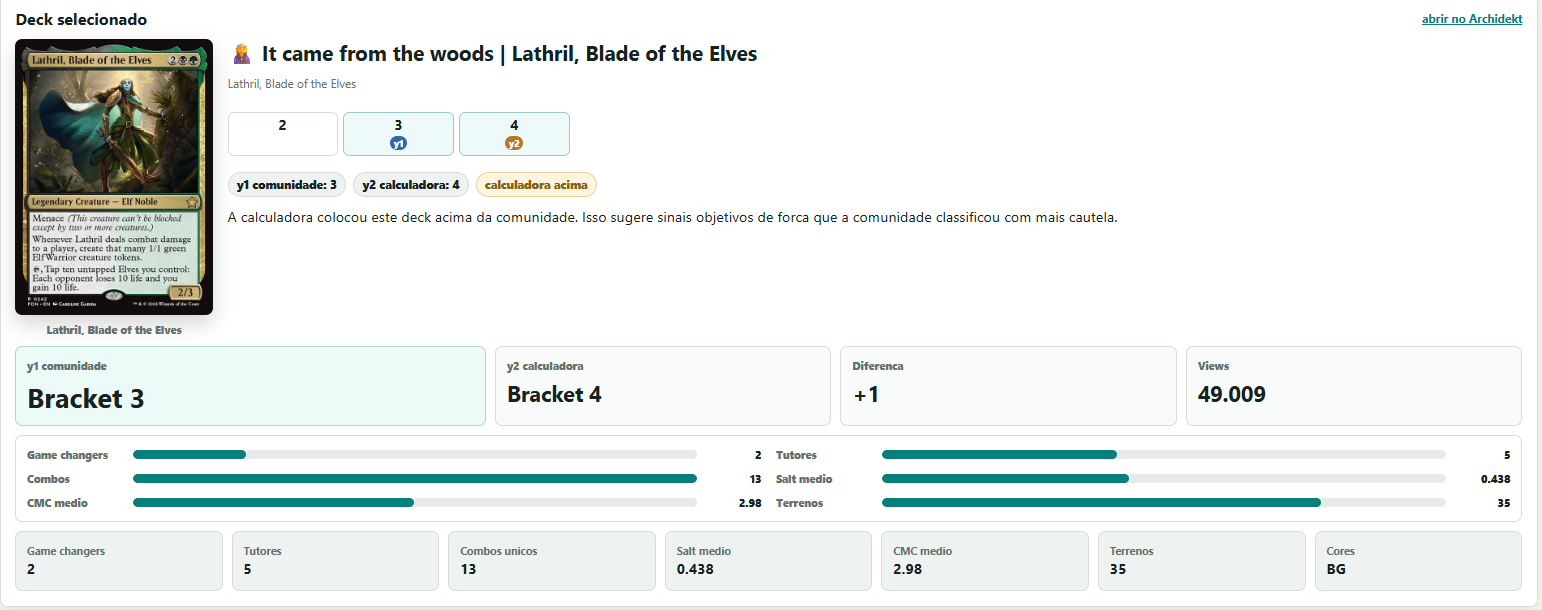
\includegraphics[width=0.66\textwidth]{figures/mtg-demo-1.png}}\\[1pt]
        \visible<5->{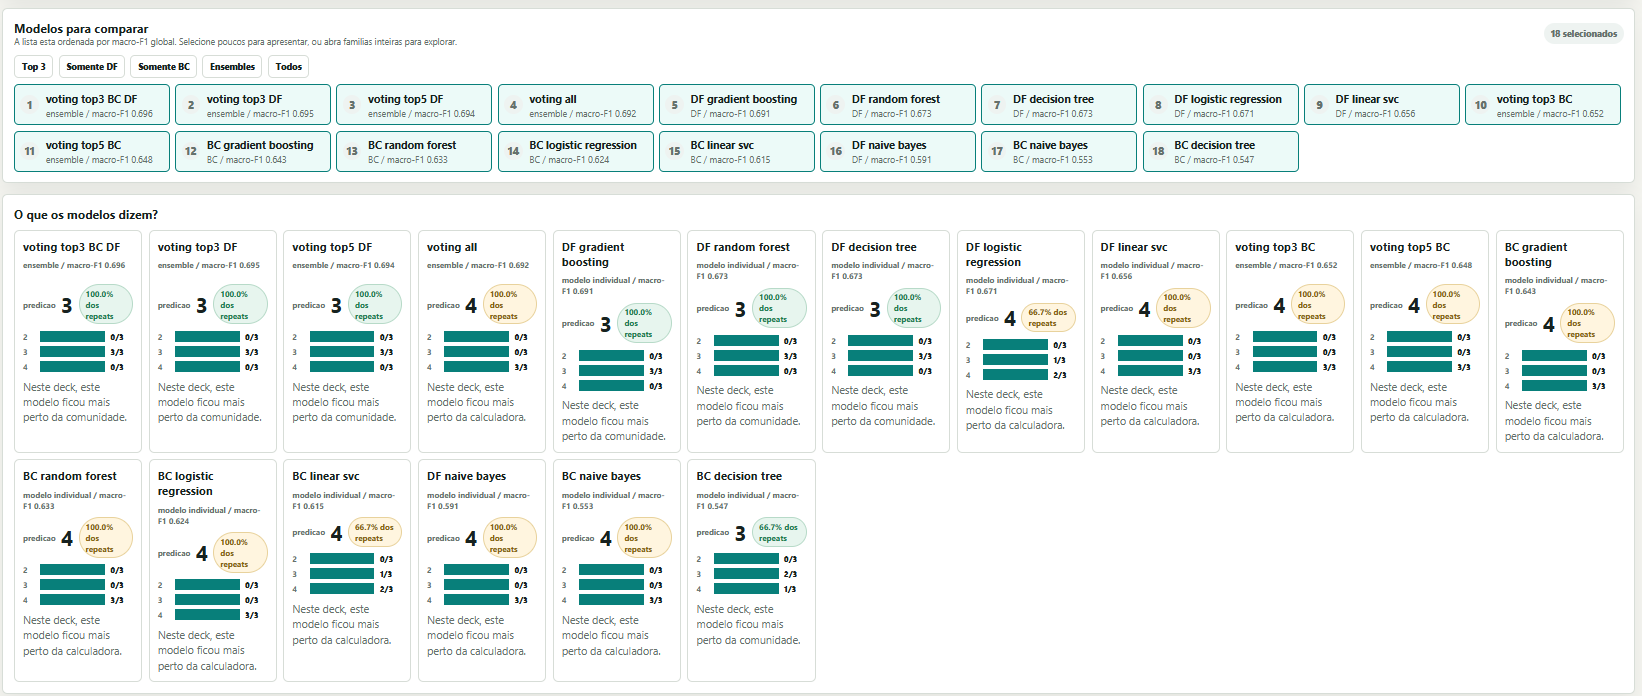
\includegraphics[width=0.66\textwidth]{figures/mtg-demo-2.png}}
    \end{center}
\end{frame}


% ============================================================
% SLIDE 15 -- Thanks (sem nomes)
% NOTA: ~15s.
% ============================================================
\begin{frame}{Thank you.}
    \vfill
    \begin{center}
        \Large \textbf{Questions?}
    \end{center}
    \vfill
\end{frame}

\end{document}
